%
================================================================
% Chapter � BDY TOOLS SETUP
%
================================================================
\chapter{Overview of BDY Tools }
\label{setup}

$\ $\newline    % force a new ligne


%gm% add here introduction to this chapter

%
\noindent ================================================================
% Boundary Condition at the Coast
%
================================================================

\section{Overview}


The BDY tools use grid information from the source data (e.g. a global NEMO 025
run) and destination simulation (i.e. the proposed regional simulation) to determine which source points are
required for data extraction. This is done using a kdtree approximate nearest
neighbour algorithm. The idea behind this targetted method is that if a NEMO
style grid file is produced (tool to be written) for non-\NEMO source data in principle the BDY tools 
become more generic. At present (alpha release) the tools do not contain many
options, but those that exist at accessed through a NEMO style namelist that is read in
when the main python call is made. The following sections summarise the inputs 
required to produce a set of BDY files to force a regional NEMO simulation.

\subsection{Boundary geometry}
\label{BDY_geometry}

Each open boundary set is defined as a list of points. The
information
is stored in the arrays $nbi$, $nbj$, and $nbr$ in the
$idx\_bdy$
structure.  The $nbi$ and $nbj$ arrays
define the local $(i,j)$ indices of each point in the boundary
zone
and the $nbr$ array defines the discrete distance from the
boundary
with $nbr=1$ meaning that the point is next to the edge of the
model domain and $nbr>1$ showing that the point is increasingly
further away from the edge of the model domain. A set of $nbi$,
$nbj$,
and $nbr$ arrays is defined for each of the $T$, $U$ and $V$
grids. Figure \ref{Fig_LBC_bdy_geom} shows an example of an
irregular
boundary. 

The boundary geometry for each set may be defined in a namelist
nambdy\_index or by reading in a ``coordinates.bdy.nc'' file.
The
nambdy\_index namelist defines a series of straight-line
segments for
north, east, south and west boundaries. For the northern
boundary,
\np{nbdysegn} gives the number of segments, \np{jpjnob} gives
the $j$
index for each segment and \np{jpindt} and \np{jpinft} give the
start
and end $i$ indices for each segment with similar for the other
boundaries. These segments define a list of $T$ grid points
along the
outermost row of the boundary ($nbr\,=\, 1$). The code deduces
the $U$ and
$V$ points and also the points for $nbr\,>\, 1$ if
$nn\_rimwidth\,>\,1$.

The boundary geometry may also be defined from a
``coordinates.bdy.nc'' file. Figure \ref{Fig_LBC_nc_header}
gives an example of the header information from such a file. The
file
should contain the index arrays for each of the $T$, $U$ and $V$grids. The
arrays must be in order of increasing $nbr$. Note
that the
$nbi$, $nbj$ values in the file are global values and are
converted to
local values in the code. Typically this file will be used to
generate
external boundary data via interpolation and so will also
contain the
latitudes and longitudes of each point as shown. However, this
is not
necessary to run the model. 

For some choices of irregular boundary the model domain may
contain
areas of ocean which are not part of the computational domain.
For
example if an open boundary is defined along an isobath, say at
the
shelf break, then the areas of ocean outside of this boundary
will
need to be masked out. This can be done by reading a mask file
defined
as \np{cn\_mask\_file} in the nam\_bdy namelist. Only one mask
file is
used even if multiple boundary sets are defined.

%>>>>>>>>>>>>>>>>>>>>>>>>>>>>
\begin{figure}[!t]      \begin{center}
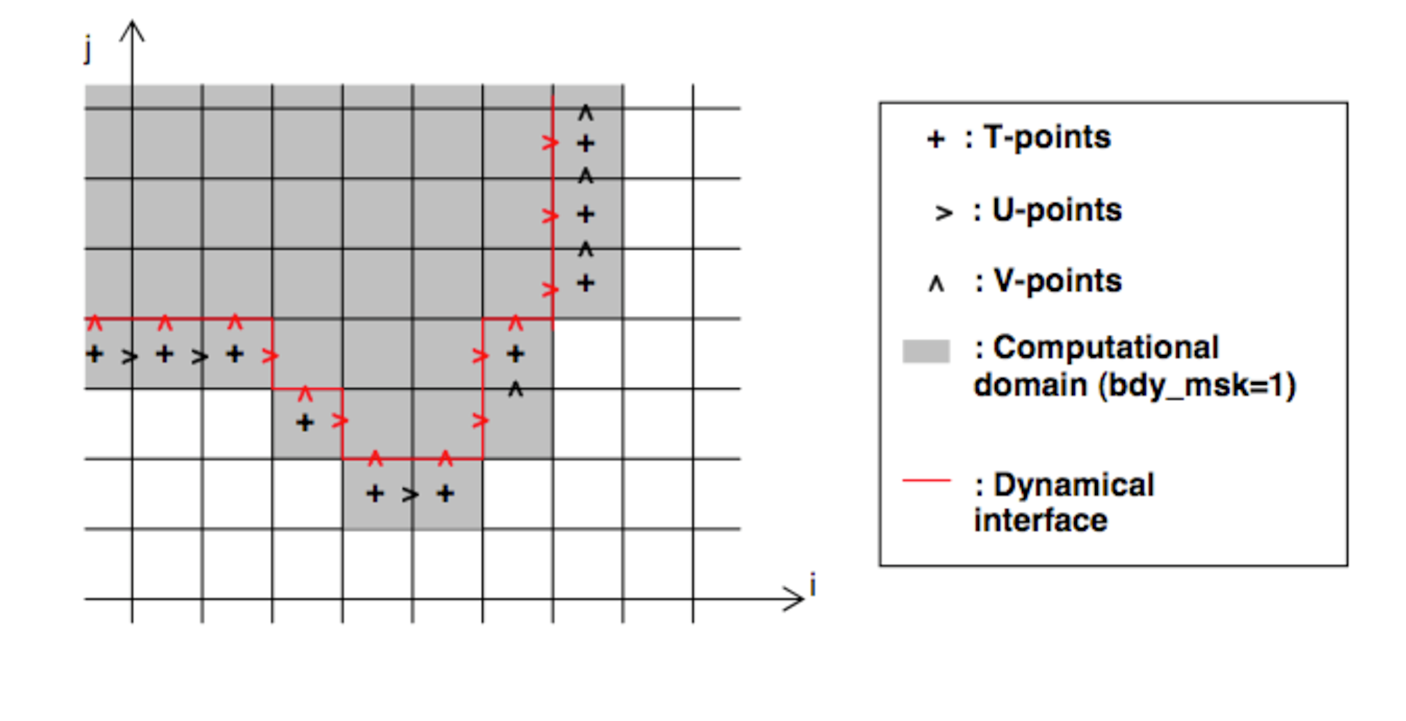
\includegraphics[width=1.0\textwidth]{./TexFiles/Figures/Fig_LBC_bdy_geom.pdf}
\caption {      \label{Fig_LBC_bdy_geom}
Example of geometry of unstructured open boundary}
\end{center}   \end{figure}
%>>>>>>>>>>>>>>>>>>>>>>>>>>>>


\subsection{Defining the regional domain}
\label{domain}

2 options:

read in mask - how is this defined : netcdf file listed in namelist? if not present gui pops up?

generate new mask using gui


\section{Grid Information}
\label{s_coord}
%--------------------------------------------namvert-------------------------------------------------------
\namdisplay{./TexFiles/Namelist/namgrd.nml} 
%--------------------------------------------------------------------------------------------------------------

There is no clean way given a coordinates.nc file and bathymetry.nc file to generate the grid information
from the proposed regional simulation, without replicating a lot of the domzgr.F90  code. At this early stage
in writing BDY tools it was deamed cleaner and safer if this information is required as input. This is easily 
achieved by running the proposed regional simulation for a single timestep with \np{nn\_msh} set to 3 in the 
\NEMO namelist file. This will output 3 files: msh\_hgr.nc, msh\_zgr.nc and mask.nc.
A mask from the source grid is also required (\np{cn\_src\_msk}). It is often the case the data have
be post processed and are missing relavent meta data to determine where the land ocean divide 
is (e.g. the land values in an ice field are set to zero). The tools rely on the masks and do not 
search for missing\_value or \_FillValue properties as these have been found to be unreliable. 
However, scale\_factor and off\_set are still read from the source files if they exist and applied to
the relevant data.

\section{Vertical coordinate}
\label{vert_coord}
%--------------------------------------------namvert-------------------------------------------------------
\namdisplay{./TexFiles/Namelist/namvert.nml} 
%--------------------------------------------------------------------------------------------------------------




\subsection{S-coordinate}
\label{s_coord}
%--------------------------------------------namvert-------------------------------------------------------
\namdisplay{./TexFiles/Namelist/namsco.nml} 
%--------------------------------------------------------------------------------------------------------------


\subsection{unstructured open boundaries options}
\label{bdyopts}




\subsection{Post Extraction}
\label{pe}
%--------------------------------------------namvert-------------------------------------------------------
\namdisplay{./TexFiles/Namelist/namextra.nml} 
%--------------------------------------------------------------------------------------------------------------

weighting gauss nearest linear bicube?
the use of weighting function - auto generate to right length? truncated by fr smoothing red
use of fr / auto? / 
fr in search and fr in smoothing
fr set to small is nearest neighbour (talk in terms of grid res + pictorial e.g.)





%----------------------------------------------

%----------------------------------------------
\subsection{Input boundary data files}
\label{BDY_data}

The data files contain the data arrays
in the order in which the points are defined in the $nbi$ and
$nbj$
arrays. The data arrays are dimensioned on: a time dimension;
$xb$ which is the index of the boundary data point in the
horizontal;
and $yb$ which is a degenerate dimension of 1 to enable the file
to be
read by the standard NEMO I/O routines. The 3D fields also have
a
depth dimension. 

At Version 3.4 there are new restrictions on the order in which
the
boundary points are defined (and therefore restrictions on the
order
of the data in the file). In particular:

\mbox{}

\begin{enumerate}
\item The data points must be in order of increasing $nbr$, ie.
all
  the $nbr=1$ points, then all the $nbr=2$ points etc.
\item All the data for a particular boundary set must be in the
same
order. (Prior to 3.4 it was possible to define barotropic data
in a
different order to the data for tracers and baroclinic
velocities).
\end{enumerate}

\mbox{}

These restrictions mean that data files used with previous
versions of
the model may not work with version 3.4. A fortran utility
{\it bdy\_reorder} exists in the TOOLS directory which will
re-order the
data in old BDY data files. 

%>>>>>>>>>>>>>>>>>>>>>>>>>>>>
\begin{figure}[!t]     \begin{center}
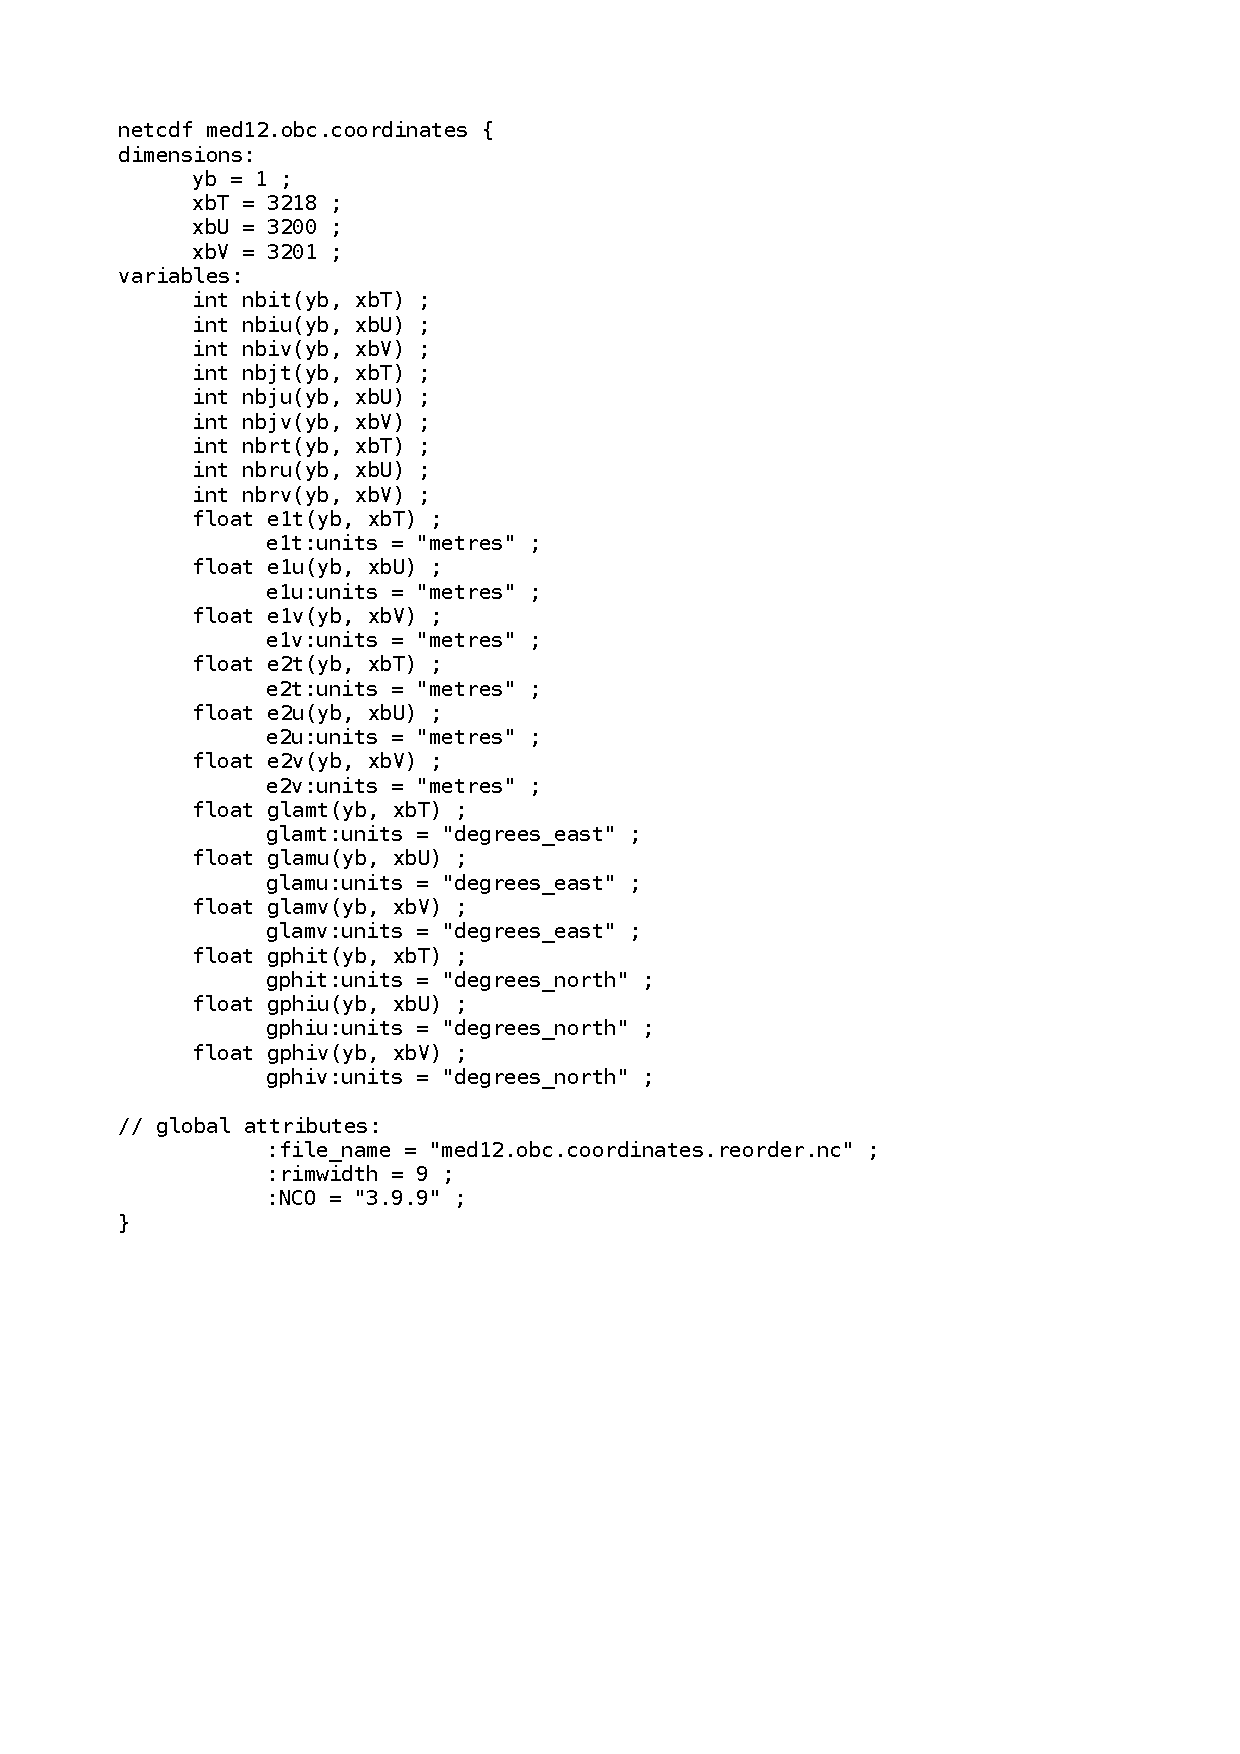
\includegraphics[width=1.0\textwidth]{./TexFiles/Figures/Fig_LBC_nc_header.pdf}
\caption {     \label{Fig_LBC_nc_header} 
Example of the header for a coordinates.bdy.nc file}
\end{center}   \end{figure}
%>>>>>>>>>>>>>>>>>>>>>>>>>>>>

%----------------------------------------------

\subsection{Debugging}
\label{Debug}


